\documentclass[12pt,a4paper,twocolumn]{article}
\title{HI LATEX}
\author{Keno}
\date{\today}
\usepackage{graphicx}

\begin{document}
\maketitle
\section{no idea}
Hi I have absolutely no idea how this will look in the document.
Therefore I am just writing some random text to text how Latex will format
text.
\section{new ideas}
Compiling this interesting document is more fun than I thought it would be and I get know why people would prefer using this system than word. It's pretty easy and straightforward with the possibility to use it in your
favorite environment.
\section{latest thoughts}
Writing this document has given me some more ideas. I kind of already like LaTeX now.
\subsection{why}
Why do I like it?
Well I really do enjoy that it's free and open-source and I can hack around it.
\subsection{additional thoughts}
I just like it.
\section{lists}
\subsection{enumerate}
\begin{enumerate}
	\item first
	\item second
	\item third
\end{enumerate}
\subsection{bulletpoint}
\begin{itemize}
	\item bored
	\item not anymore
	\item still?
\end{itemize}
\section{cad}
You might ask: What do you do on a wednesday afternoon?
Well this is what I have done on a wednesday afternoon:
\begin{figure}[h]
	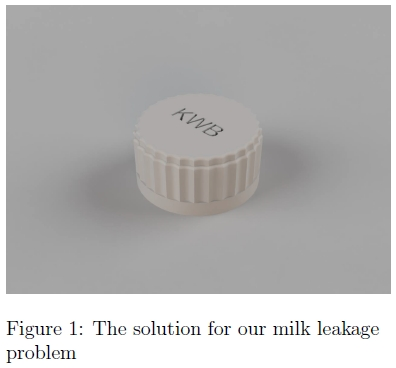
\includegraphics[width=80mm]{/dcs/16/u1632823/Downloads/cad.png}
	\caption{The solution for our milk leakage problem}
	\label{reflabel}
\end{figure}
\section{random new stuff}
\begin{equation}
	a^{2} - b^{2} = (a-b)(a+b)
	\label{diff2squares}
\end{equation}
\end{document}
